% Options for packages loaded elsewhere
\PassOptionsToPackage{unicode}{hyperref}
\PassOptionsToPackage{hyphens}{url}
%
\documentclass[
]{article}
\usepackage{lmodern}
\usepackage{amsmath}
\usepackage{ifxetex,ifluatex}
\ifnum 0\ifxetex 1\fi\ifluatex 1\fi=0 % if pdftex
  \usepackage[T1]{fontenc}
  \usepackage[utf8]{inputenc}
  \usepackage{textcomp} % provide euro and other symbols
  \usepackage{amssymb}
\else % if luatex or xetex
  \usepackage{unicode-math}
  \defaultfontfeatures{Scale=MatchLowercase}
  \defaultfontfeatures[\rmfamily]{Ligatures=TeX,Scale=1}
\fi
% Use upquote if available, for straight quotes in verbatim environments
\IfFileExists{upquote.sty}{\usepackage{upquote}}{}
\IfFileExists{microtype.sty}{% use microtype if available
  \usepackage[]{microtype}
  \UseMicrotypeSet[protrusion]{basicmath} % disable protrusion for tt fonts
}{}
\makeatletter
\@ifundefined{KOMAClassName}{% if non-KOMA class
  \IfFileExists{parskip.sty}{%
    \usepackage{parskip}
  }{% else
    \setlength{\parindent}{0pt}
    \setlength{\parskip}{6pt plus 2pt minus 1pt}}
}{% if KOMA class
  \KOMAoptions{parskip=half}}
\makeatother
\usepackage{xcolor}
\IfFileExists{xurl.sty}{\usepackage{xurl}}{} % add URL line breaks if available
\IfFileExists{bookmark.sty}{\usepackage{bookmark}}{\usepackage{hyperref}}
\hypersetup{
  pdftitle={SCBI-ForestGEO Tree Health and Mortality Census Protocol 2021},
  hidelinks,
  pdfcreator={LaTeX via pandoc}}
\urlstyle{same} % disable monospaced font for URLs
\usepackage[margin=1in]{geometry}
\usepackage{graphicx}
\makeatletter
\def\maxwidth{\ifdim\Gin@nat@width>\linewidth\linewidth\else\Gin@nat@width\fi}
\def\maxheight{\ifdim\Gin@nat@height>\textheight\textheight\else\Gin@nat@height\fi}
\makeatother
% Scale images if necessary, so that they will not overflow the page
% margins by default, and it is still possible to overwrite the defaults
% using explicit options in \includegraphics[width, height, ...]{}
\setkeys{Gin}{width=\maxwidth,height=\maxheight,keepaspectratio}
% Set default figure placement to htbp
\makeatletter
\def\fps@figure{htbp}
\makeatother
\setlength{\emergencystretch}{3em} % prevent overfull lines
\providecommand{\tightlist}{%
  \setlength{\itemsep}{0pt}\setlength{\parskip}{0pt}}
\setcounter{secnumdepth}{-\maxdimen} % remove section numbering
\ifluatex
  \usepackage{selnolig}  % disable illegal ligatures
\fi

\title{SCBI-ForestGEO Tree Health and Mortality Census Protocol 2021}
\author{}
\date{\vspace{-2.5em}}

\begin{document}
\maketitle

\hypertarget{supplies}{%
\subsection{Supplies}\label{supplies}}

\begin{itemize}
\tightlist
\item[$\square$]
  iPad - set up with FastField and maps
  (\href{https://github.com/SCBI-ForestGEO/SCBImortality/issues/6}{GitHub
  issue \#6})
\item[$\square$]
  DBH tape, calipers
\item[$\square$]
  Binoculars, IMPORTANT to check live status of very tall trees and to
  distinguish between leaves of lianas or tree under inspection.
\item[$\square$]
  Printed copies of visual guides, if desired (these could also be
  loaded on iPad)
\item[$\square$]
  Personal gear/ safety equipment
\end{itemize}

\hypertarget{procedure}{%
\subsection{Procedure}\label{procedure}}

\hypertarget{plot-navigation-tree-location}{%
\subsubsection{Plot Navigation \& Tree
Location}\label{plot-navigation-tree-location}}

At the SCBI plot, a blue re-bar located in the SW corner gives the
quadrat name (3 or 4 digits). Locate the rebar and orientate yourself
(N-S). Locate all trees within the quadrat you are working on and make
sure you complete all trees before moving to the next quadrat.
Coordinates (x, y) are given in reference to a 20x20m square.

Review info (species, size, position) of tree for which you're
searching. Locate the based on x-y coordinates and/or map, check tag to
ensure you've got the right tree.

\emph{If you can't find a tree:} (1) double check that quadrat matches
data sheet/ Fastfield App (2) look on the ground for fallen trees/ lost
tags (3) sometimes x and y coordinates get switched, so try switching
and see if you find it (note wrong coordinates) (4) check trees that
otherwise don't seem to match what you're looking for (5) if a thorough
search yields nothing, record as \textbf{DN} (no plant nor tag found)
Avoid giving a tree the DN status; you need to do a thorough search for
all trees on the list.

\hypertarget{data-entry-in-fastfield}{%
\subsubsection{Data Entry in FastField}\label{data-entry-in-fastfield}}

\hypertarget{tree-classification}{%
\subsubsection{Tree Classification}\label{tree-classification}}

\emph{If the status us ``A'':} (1) Mark status (2) Record crown position
(3) Record percentage of crown still intact (\%) (4) Record percentage
of crown living

\emph{If the status is ``AU''} AU is used for trees that are alive but
noticeably unhealthy (e.g., fallen and uprooted but not yet dead,
wounded, insect damage).

(1)Record FADs in order of importance* (at least 1 factor)- See FAD
codes below. (2) Record crown position. (3) Record percentage of crown
still intact (\%). (4) Record percentage of crown living (5) Record lean
angle (if leaning \textgreater{} 15°) (6) Record Liana load. (7) Record
wound, canker, or rot categories (if applicable) (8) Take pictures: Take
a picture of alive unhealthy tree if picture appropriately captures FAD.
For example, take picture of wounds to main bole, but not of leaf damage
high in canopy. Take a picture of the tag first then make 2-3 pics of
main FADS. Make nice close-ups if any insect or insect galleries are
found.

\hypertarget{in-fastfieldforms-click-fad-in-order-of-importance}{%
\subsubsection{*In FastFieldForms, click FAD in order of
importance}\label{in-fastfieldforms-click-fad-in-order-of-importance}}

\emph{If the status is ``DS'' \& previously ``A'':} (1) Record FADs in
order of importance (at least 1 factor)- See FAD codes below. (2) Record
crown position. (3) Record Percentage of crown still intact (\%). (4)
Record percentage of crown living (\%) (5) Record lean angle (if leaning
\textgreater{} 15°) (6) Record Liana load. (7) Record wound, canker, or
rot categories (if applicable) (8) Take pictures: Take a picture of dead
tree if picture appropriately captures FAD. Take a picture of the tag
first then make 2-3 pics of main FADS. Make nice close-ups if any insect
or insect galleries are found.

\emph{If the status is ``DG'' \& previously ``A'':}

\begin{enumerate}
\def\labelenumi{(\arabic{enumi})}
\tightlist
\item
  Record FADs in order of importance (at least 1 factor)- See FAD codes
  below.
\item
  Record Percentage of crown still intact (\%).
\item
  Record percentage of crown living (\%)
\item
  Record Liana load.
\item
  Record wound, canker, or rot categories (if applicable)
\item
  Take pictures: Take a picture of dead tree if picture appropriately
  captures FAD. Take a picture of the tag first then make 2-3 pics of
  main FADS. Make nice close-ups if any insect or insect galleries are
  found.
\end{enumerate}

--Note: for stems that were ``A'' and now ``DG'' (typically uncommon) it
is unnecessary to record canopy position

\emph{If the status is ``DS'' \& previously ``DS'':} (1) Mark status (2)
Record crown position\emph{. (3) Record percentage of crown still intact
(\%)} (4) Record percentage of crown living (\%)\emph{ (5) Record lean
angle (if leaning \textgreater{} 15°)} (6) Record Liana load\emph{.
}record this information for remote sensing/crown delineation purposes

\emph{If the status is ``DG'' \& previously ``DS''}\\
Record status and continue.

\hypertarget{additional-fields}{%
\subsubsection{--Additional Fields--}\label{additional-fields}}

\#\#\#\emph{Lean angle (\%)} If tree is still rooted and is leaning,
estimate the angle of lean in degrees from vertical. This angle is
measured in degrees from the base through the POM (see figure below).
\#\#\#\emph{Liana load (levels: 0 -- 4)} 0 = lianas absent 1 = up to
25\% of the tree crown covered by lianas 2 = 26--50\% liana cover 3 =
51--75\% liana cover 4 = 76--100\% liana cover.

\#\#\#\emph{Wounded main axis (levels: 1 = small, 2 = large, 3 =
massive)---figure below} 1 = small damage, smaller in area than a square
of DBH  DBH in shape. 2 = large damage, greater in area than a square
of DBH  DBH in shape. 3 = massive damage, affecting \textgreater50\% of
the basal area (i.e., a very deep and extensive wound; Figure 8c) or
\textgreater50\% of the living length (Figure 8d). These are cases of
main stem breakage in which the breakage is not complete and the broken
part is still connected and alive, and trunks that have been
longitudinally split in two.

\#\#\#\emph{Canker, swelling, deformity (levels: 1 = small, 2 = large, 3
= massive)} 1 = small deformity area, smaller in area than a square of
DBH  DBH in shape. 2 = big deformity, greater in area than a square of
DBH  DBH in shape. 3 = massive deformity or canker, greater than
\textgreater50\% of the basal area or \textgreater50\% of the main axis
length.

\#\#\#\emph{Rotting trunk (levels: 1 = small, 2 = large, 3 = massive)} 1
= small rotting area, smaller in area than a square of DBH  DBH in
shape. 2 = big rotting area, greater in area than a square of DBH  DBH
in shape. 3 = massive rotting, affecting \textgreater50\% of the basal
area or \textgreater50\% of the main axis length.

\textbf{Important notes:}

\begin{itemize}
\tightlist
\item
  If a tree is recorded as Alive unhealthy (\textbf{AU}) or dead, there
  should always be at least one factor associated with death (FAD)
  recorded, and photos should be taken
\item
  Record Factors associated with death (FAD) \textbf{\emph{in order of
  importance}} (will be listed in order selected).
\item
  Sometimes a tree recorded dead in a previous year is ``back to life''.
  If a dead tree is alive in the current census (meaning you are 100\%
  sure it is alive), mark the tree as \textbf{A} or \textbf{AU} and make
  a note in comments.
\item
  Measure DBH on trees that have died. If a stem has fallen and it's DBH
  can't be measured with a tape, measure it later using a big caliper
  (find one in Radiotracking lab - Office Annex building).
\item
  Take pictures: Take a picture of every unhealthy or dead tree found.
  Include photos of all factors associated with death (FADs). Make nice
  close-ups if any insect or insect galleries are found.
\item
  For tree conditions or agents of mortality not specifically defined
  below, record diagnosis in the notes or comments section of the form.
\end{itemize}

\hypertarget{identifying-factors-associated-with-death-fads}{%
\subsubsection{Identifying Factors Associated with Death
(FADs)}\label{identifying-factors-associated-with-death-fads}}

To scrutinize the FAD's, look at our
\href{https://github.com/SCBI-ForestGEO/SCBImortality/blob/main/Protocols/Visual\%20guides/Tree\%20Mortality\%20Guide_2020.pdf}{Visual
Guides}.

\hypertarget{emerald-ash-borer-add-ons}{%
\subsubsection{Emerald Ash Borer
Add-ons}\label{emerald-ash-borer-add-ons}}

\begin{itemize}
\tightlist
\item
  Estimate crown thinning via visual assessment per Smith/Flower 2013
  (see figure)
\item
  If DE are present then count all visible D-shaped holes around the
  circumference of the tree in an area 50 cm high at breast height and
  record this number. At SCBI almost all tags are located at 1.3 m, so
  use the tag as reference to visually define the 50 cm area. That is,
  search for DE all the way around the tree between 1.05 and 1.55m
  height.
\end{itemize}

\newpage

\hypertarget{codes}{%
\subsection{Codes}\label{codes}}

\textbf{\emph{Mortality census status codes:}} \textbf{A}: Alive and
healthy \textbf{AU}: Alive unhealthy \textbf{DS}: Dead, stem standing,
\textbf{DC}: Dead, stem fallen, \textbf{DT}: Only tag found,
\textbf{DN}: No plant nor tag found.

\emph{(See
\href{https://github.com/SCBI-ForestGEO/SCBImortality/issues/8}{GitHub
issue \#8} regarding Ash codes)}

\textbf{\emph{Core census codes:}} \textbf{A}: alternate pom (point of
measurement), \textbf{B}: stem broken above breast height, \textbf{C}:
dead above 1.3m, \textbf{DS}: Dead, stem standing, \textbf{DC}: Dead,
stem fallen, \textbf{DT}: Only tag found, \textbf{DN}: No plant nor tag
found. \textbf{F}: Incorporated into fence, \textbf{G}: ID to Genus
certain, \textbf{I}: stem irregular where measured, \textbf{J}: Bent,
\textbf{L}: leaning stem, \textbf{M}: multiple stems, \textbf{main};
main stem, \textbf{P}: prostrate stem, \textbf{S}: secondary stem,
\textbf{V}: Vine, \textbf{X}: stem broken below 1.3 m.

\textbf{\emph{DBH (mm)}}: Diameter at breast height in millimeters.
Given for all trees as last core census.

\textbf{\emph{Crown Position:}} \textbf{Dominant (D)}: Crown extends
above the general level of the canopy receiving full sunlight.
\textbf{Codominant (CD)}: Crown forms main level of canopy, tree
receives full sunlight from above. \textbf{Intermediate (I)}: Shorter
trees with smaller crowns, receive little light from above and none from
sides. \textbf{Suppressed (S)}: Crown below canopy, small crown receives
no direct light. \textbf{Open grown (OG)}: Crown on open areas of the
stand.

\textbf{\emph{Record Liana load}}

0 = lianas absent 1 = up to 25\% of the tree crown covered by lianas 2 =
26--50\% liana cover 3 = 51--75\% liana cover 4 = 76--100\% liana cover.

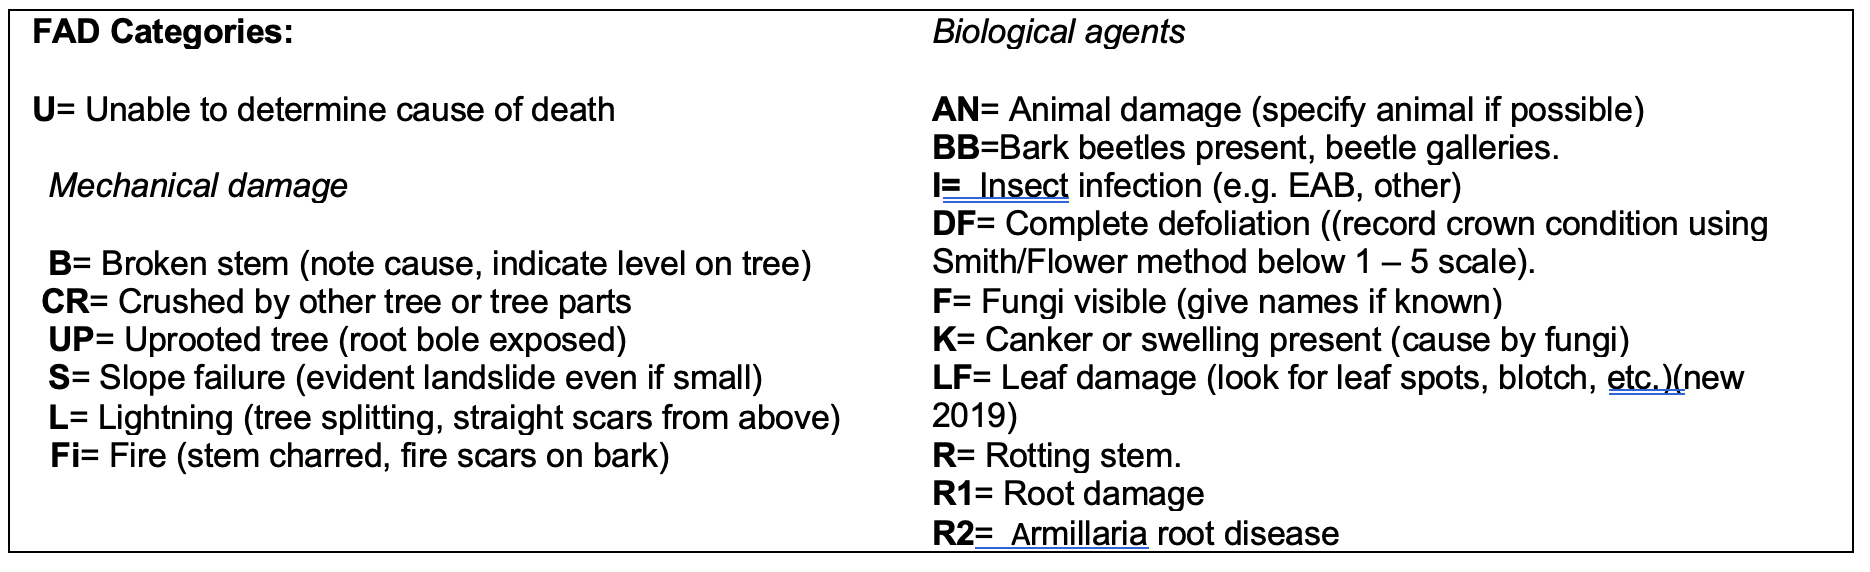
\includegraphics{figures_tables/FAD table.png}
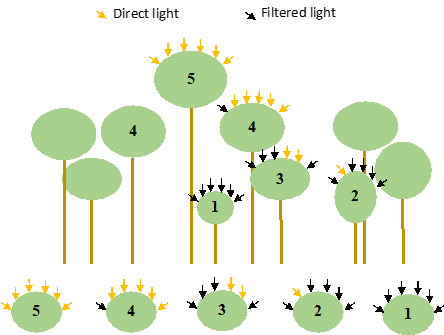
\includegraphics{figures_tables/Crown_illumination.png} 5 = Canopy
completely exposed to overhead and lateral light 4 = Full overhead
light; \textgreater{} 90\% exposed to vertical light 3 = some overhead
light 2 = Lateral light; \textless{} 10\% exposed to vertical light 1 =
No direct light; only receives light filtered through other trees

\newpage

\textbf{\emph{Lean angle (Taken from Arellano et al., 2020)}}
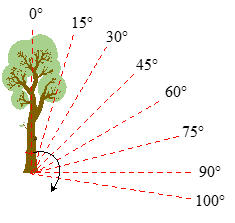
\includegraphics{figures_tables/Tree_angle.png} \#\#\# EAB census
add-ons
(\href{https://github.com/SCBI-ForestGEO/SCBImortality/issues/5}{GitHub
issue \#5})

\textbf{\emph{EAB crown thinning}}

\begin{figure}
\centering
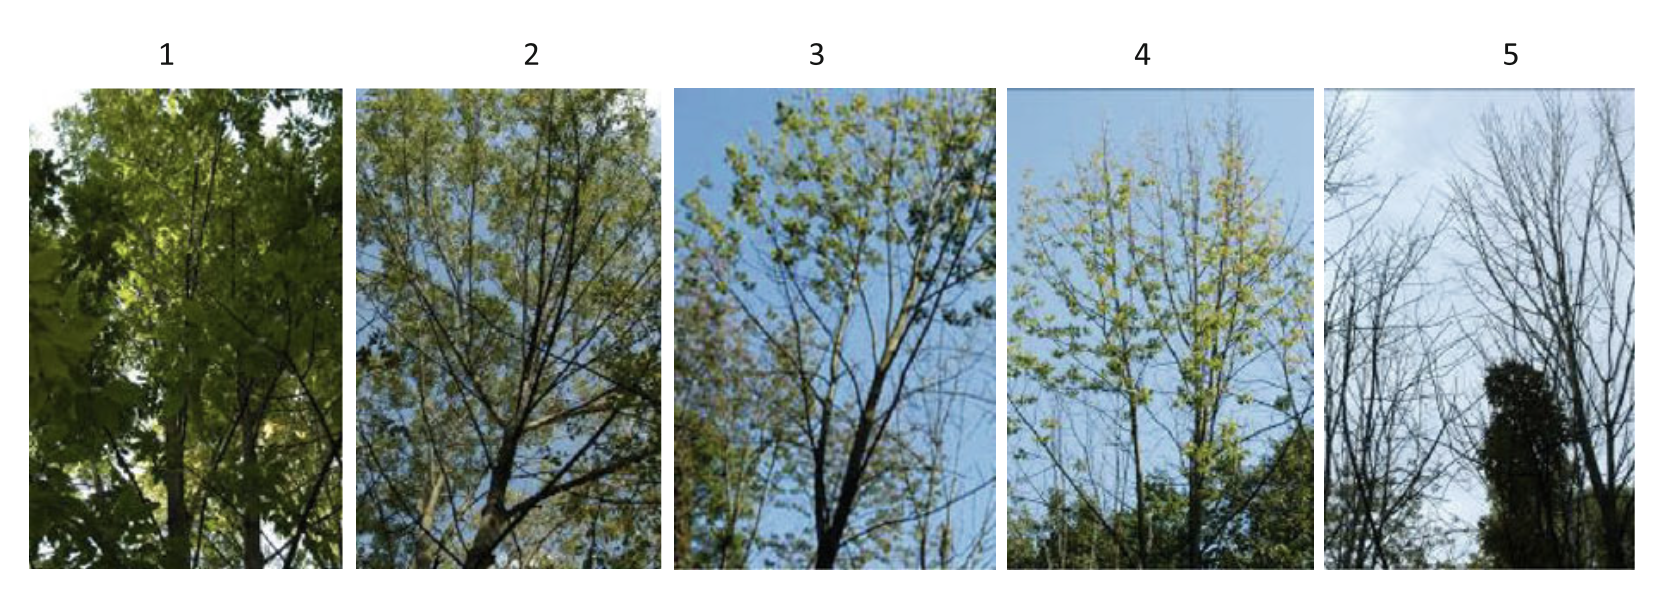
\includegraphics{figures_tables/Ash_crown_assessment.png}
\caption{Guide to estimating EAB crown thinning via visual assessment
per Smith/Flower 2013:}
\end{figure}

\textbf{1} = healthy tree with no symptoms of decline, no defoliation
\textbf{2} = slight reduction in leaf density (thinning), yet all top
branches exposed to sunlight have leaves \textbf{3} = thinning canopy
and some top branches exposed to sunlight are defoliated (\textless50\%
dieback) \textbf{4} = \textgreater50\% defoliation/dieback \textbf{5} =
Dead tree with no leaves in canopy (excluding epicormic sprouting)
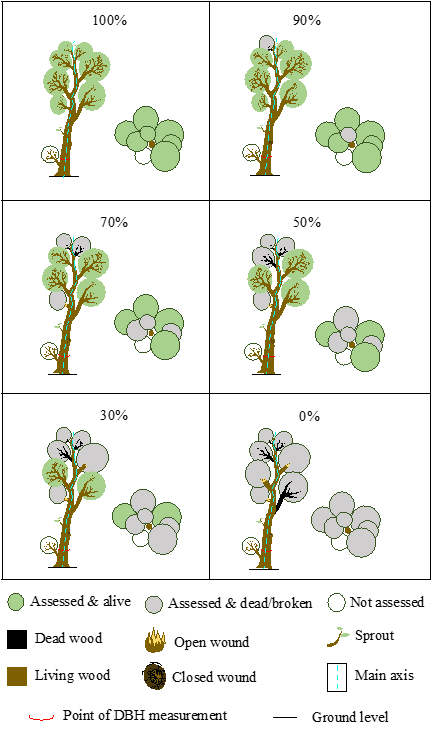
\includegraphics{figures_tables/Crown_assessment.png} Crown assessment
(taken from Arellano et al., 2020). Top left is 100\% crown intact and
100\% crown living, top right---100\% intact and 90\% living, middle
left---90\% intact and 70\% living, middle right---90\% intact and 50\%
living, bottom left---70\% intact and 30\% living, bottom right---40\%
intact and 0\% living

\textbf{\emph{Schematic of wound size (taken from Arellano et al.,
2020)}} 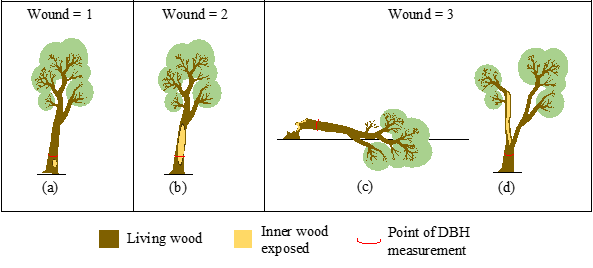
\includegraphics{figures_tables/Woundsize.png} \newpage
\textbf{\emph{Epicormics}}

\begin{figure}
\centering
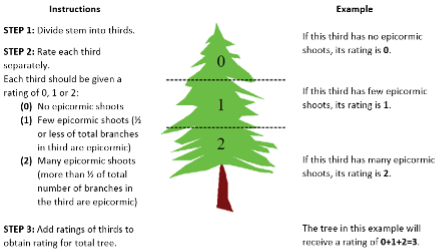
\includegraphics{figures_tables/epicormics_assessment.png}
\caption{6-class dwarf mistletoe rating system (Hawksworth 1977) to
evaluate epicormic growth}
\end{figure}

\textbf{\emph{EABF (Emerald Ash Borer Factors):}} \textbf{VB} = Vertical
bark splitting, \textbf{SS} = Stump sprouts, \textbf{AS} = Ash snap of
the branches/limbs, \textbf{W} = Bark blonding from woodpecker
predation. In comment section, write percentage estimate. \textbf{DE} =
D-shaped exit hole presence.

\newpage

\hypertarget{coring-of-dead-trees}{%
\subsection{Coring of Dead Trees}\label{coring-of-dead-trees}}

If time allows, cores will be taken at the end of survey and saved for
future analyses.

\emph{Target species}: ceca, amar, cofl, ploc, prav, rops, saal, and all
Quercus.

Follow steps in document ``Coring\_instructions\_SCBI'' located in
`Protocol' folder.

\emph{We will need to take data on trees cored (instructions to be
determined later).}

\hypertarget{changes-from-previous-years}{%
\subsection{Changes from previous
years}\label{changes-from-previous-years}}

\begin{itemize}
\tightlist
\item
  Adding some measurements to align with censuses at other plots under
  NSF Macrosystems grant (PI Johnson)
\item
  Some categorical measurements are replaced with more specific
  measurements: e.g., categories for percentage crown intact replaced
  with continuous estimate.
\item
  Switching from manual data entry in spreadsheet (iPad spreadsheet or,
  previously, printed data sheets) to FastField App
\item
  Starting data checking with continuous integration
\item
  No coring of dead trees during census (if time allows, it will be done
  once survey is completed)
\end{itemize}

\end{document}
